\documentclass[a4paper,10pt,abstracton]{scrartcl}

\usepackage[margin=2.5cm]{geometry}
\usepackage{graphicx}
\usepackage[UKenglish]{babel}
\usepackage{csquotes}
\usepackage[style=numeric,citestyle=numeric,backend=biber,sorting=none,doi=false,url=false]{biblatex}
\usepackage{float}
\usepackage[export]{adjustbox}
\usepackage[T1]{fontenc}
\usepackage{lmodern}
\usepackage{todonotes}
\usepackage[labelsep=period,font=small,labelfont=bf,format=plain]{caption}
\usepackage[group-separator={,}]{siunitx}
\usepackage{booktabs}
\usepackage{pdflscape}
\usepackage{tablefootnote}
\usepackage{authblk}

\addbibresource{refs.bib}

\title{
The genetic architecture of target-site resistance to DDT and pyrethroids in the malaria vectors \emph{Anopheles gambiae} and \emph{Anopheles coluzzii}
}

\subtitle{DRAFT}

\author[1]{Chris S. Clarkson}
\author[2,1]{Alistair Miles}
\author[2]{Nicholas J. Harding}
\author{@@TODO}
\author[1,2]{Dominic Kwiatkowski}
\author[3,1]{Martin Donnelly}
\author[4]{The \emph{Anopheles gambiae} 1000 Genomes Consortium}
\affil[1]{Sanger @@TODO}
\affil[2]{Oxford @@TODO}
\affil[3]{Liverpool @@TODO}
\affil[4]{MalariaGEN @@TODO}

\begin{document}

\maketitle

\begin{abstract}

%%
TODO edits from Chris...
%
this is a drill, this is a drill

\end{abstract}

\section*{Introduction}

%%
The malaria vectors \emph{Anopheles gambiae} and \emph{Anopheles coluzzii} are evolving insecticide resistance.
%
Asdlkj dsalkj daslkjd aslkjdas lkadsj lkadsj adslkj adslkja dslkadsj lkadsj lkasd jlkadsj lkads jlakds alksdj asdlk jasdlk adslk jadslkj adslkj adslkj adslkj adslkj adslk jasd.

%%
This is the second paragraph of the introduction.
%
Asdlkjio weipo ewrpoi ewrpoi rwepoi werpoiwre poi rewpoi rwepoi erwpoi rewpoi rwepoi rwepoi rwepoi rewpo iwrepoi rwepoi wrepoi wrepoi rwpeo irwpo irwepoi rwepo ipoewi rpow ierwe.

%%
Third paragraph zcx,m ncxz,mxczn ,mxczn,mxcz n,mcnxz ,mxczn ,mz ncx,mzcxn.

%%
Fourth paragraph asdlkj dsakljdsalkj dsalkj daslkj daslkj dsalkj daslkj sda \cite{Garud2015}.

%%
TODO xz,m.cxzm.,czx.,m czx.,m zcx.,m czx.,m czx.,m zcx.

\section*{Results}

%%
Let's add some results qweoi qewoiewqoip peqwpoi ewqpoi ewqpoieqwipo ewqipo eqwpio eqwipo ewqoip ewqoip ewqiop eqw.

%%
Isn't Figure \ref{fig:demo} interesting! 
%
Table \ref{table:demo} is pretty interesting too.

\begin{landscape}
\begin{table}[h]
  \small
  \centering
  
\begin{tabular}{lllrrrrrrrrrrr}
\toprule
\multicolumn{3}{c}{Mutation} &
\multicolumn{9}{c}{Population allele frequency (\%)} &
\multicolumn{2}{c}{LD ($D'$)} \\
\cmidrule(r){1-3}
\cmidrule(r){4-12}
\cmidrule(r){13-14}
Position\tablefootnote{Position relative to AgamP3 reference sequence, chromosome arm 2L.} & 
\emph{Ag}\tablefootnote{Codon numbering according to transcript \texttt{AGAP004707-RA} in geneset AgamP4.4.} & 
\emph{Md}\tablefootnote{Codon numbering according to \emph{Musca domestica Vgsc} EMBL accession X96668 \cite{williamson1996}.} & 
AO\emph{Ac} & 
BF\emph{Ac} & 
GN\emph{Ag} & 
BF\emph{Ag} & 
CM\emph{Ag} & 
GA\emph{Ag} & 
UG\emph{Ag} & 
KE & 
GW & 
\texttt{L995S} & 
\texttt{L995F} \\
\midrule

\texttt{2,390,177 G>A} & \texttt{R254K} & \texttt{R261} & 0 & 0 & 0 & 0 & 32 & 21 & 0 & 0 & 0 & -0.98 & 0.96 \\

\texttt{2,391,228 G>C} & \texttt{V402L} & \texttt{V410} & 0 & 7 & 0 & 0 & 0 & 0 & 0 & 0 & 0 & -1 & -0.41 \\

\texttt{2,391,228 G>T} & \texttt{V402L} & \texttt{V410} & 0 & 7 & 0 & 0 & 0 & 0 & 0 & 0 & 0 & -1 & 0.10 \\

\texttt{2,399,997 G>C} & \texttt{D466H} & \texttt{-} & 0 & 0 & 0 & 0 & 7 & 0 & 0 & 0 & 0 & -1 & 1 \\

\texttt{2,400,071 G>A} & \texttt{M490I} & \texttt{M508} & 0 & 0 & 0 & 0 & 0 & 0 & 0 & 18 & 0 & -0.33 & -1 \\

\texttt{2,400,071 G>T} & \texttt{M490I} & \texttt{M508} & 0 & 0 & 0 & 0 & 0 & 0 & 0 & 0 & 0 & -1 & -0.01 \\

\texttt{2,416,980 C>T} & \texttt{T791M} & \texttt{T810} & 0 & 1 & 13 & 14 & 0 & 0 & 0 & 0 & 0 & -1 & 1 \\

\texttt{2,422,651 T>C} & \texttt{L995S} & \texttt{L1014} & 0 & 0 & 0 & 0 & 15 & 64 & 100 & 76 & 0 & 1 & -1 \\

\texttt{2,422,652 A>T} & \texttt{L995F} & \texttt{L1014} & 86 & 85 & 100 & 100 & 53 & 36 & 0 & 0 & 0 & -1 & 1 \\

\texttt{2,424,384 C>T} & \texttt{A1125V} & \texttt{K1133} & 9 & 0 & 0 & 0 & 0 & 0 & 0 & 0 & 0 & -1 & -1 \\

\texttt{2,425,077 G>A} & \texttt{V1254I} & \texttt{I1262} & 0 & 0 & 0 & 0 & 0 & 0 & 0 & 0 & 5 & -1 & -1 \\

\texttt{2,429,617 T>C} & \texttt{I1527T} & \texttt{I1532} & 0 & 14 & 0 & 0 & 0 & 0 & 0 & 0 & 0 & -1 & -1 \\

\texttt{2,429,745 A>T*} & \texttt{N1570Y} & \texttt{N1575} & 0 & 26 & 10 & 22 & 6 & 0 & 0 & 0 & 0 & -1 & 0.98 \\

\texttt{2,429,897 A>G} & \texttt{E1597G} & \texttt{E1602} & 0 & 0 & 6 & 4 & 0 & 0 & 0 & 0 & 0 & -1 & 1 \\

\texttt{2,429,915 A>C} & \texttt{K1603T} & \texttt{K1608} & 0 & 5 & 0 & 0 & 0 & 0 & 0 & 0 & 0 & -1 & 1 \\

\texttt{2,430,424 G>T} & \texttt{A1746S} & \texttt{A1751} & 0 & 0 & 11 & 13 & 0 & 0 & 0 & 0 & 0 & -1 & 1 \\

\texttt{2,430,817 G>A} & \texttt{V1853I} & \texttt{V1858} & 0 & 0 & 8 & 5 & 0 & 0 & 0 & 0 & 0 & -1 & 1 \\

\texttt{2,430,863 T>C} & \texttt{I1868T} & \texttt{I1873} & 0 & 0 & 18 & 25 & 0 & 0 & 0 & 0 & 0 & -1 & 1 \\

\texttt{2,430,880 C>T} & \texttt{P1874S} & \texttt{P1879} & 0 & 21 & 0 & 0 & 0 & 0 & 0 & 0 & 0 & -1 & 1 \\

\texttt{2,430,881 C>T} & \texttt{P1874L} & \texttt{P1879} & 0 & 7 & 45 & 26 & 0 & 0 & 0 & 0 & 0 & -1 & 1 \\

\texttt{2,431,061 C>T} & \texttt{A1934V} & \texttt{A1939} & 0 & 12 & 0 & 0 & 0 & 0 & 0 & 0 & 0 & -1 & 1 \\

\texttt{2,431,079 T>C} & \texttt{I1940T} & \texttt{I1945} & 0 & 4 & 0 & 0 & 7 & 0 & 0 & 0 & 0 & -1 & 1 \\

\bottomrule
\end{tabular}

  \caption{
\textbf{Non-synonymous mutations in the voltage-gated sodium channel gene}. 
%
All mutations are at 5\% frequency or above in one or more of the 9 Ag1000G phase 1 populations, with the exception of \texttt{2,400,071 G>T} which is only found in the CM\emph{Ag} population at 0.4\% frequency but is included because another mutation (\texttt{2,400,071 G>A}) is found at the same position causing the same amino acid substitution (\texttt{M490I}). 
%
Substitutions marked with an asterisk (*) failed conservative variant filters applied genome-wide in the Ag1000G phase 1 AR3 callset, but appeared sound on manual inspection of read alignments.
}
  \label{table:variants_missense}
\end{table}
\end{landscape}

\begin{figure}[t!]
  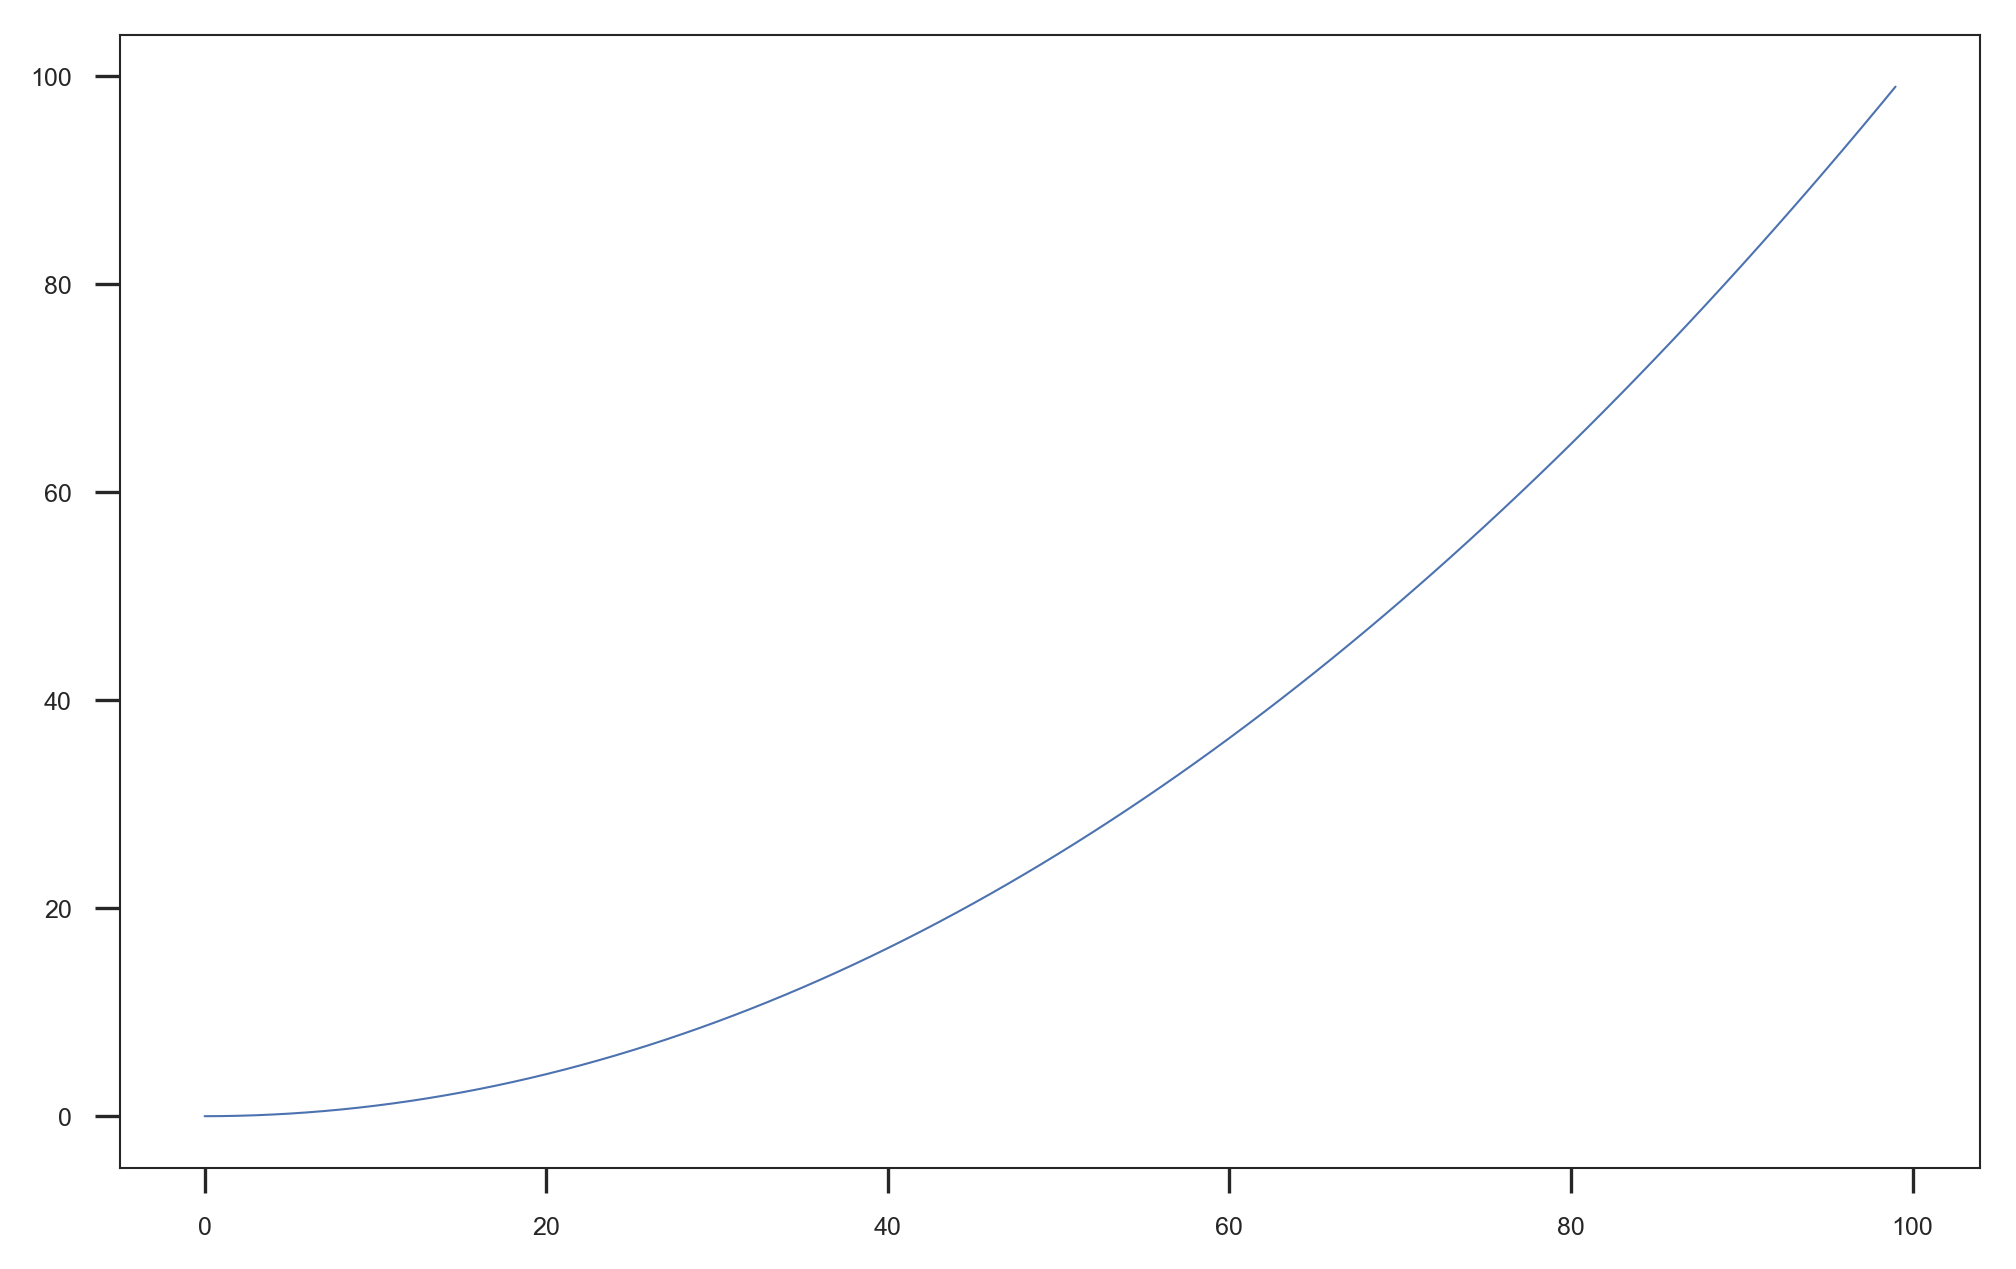
\includegraphics[width=1.1\linewidth,center]{artwork/demo.png}
  \caption{Demo figure.}
  \label{fig:demo}
\end{figure}

TODO

\begin{table}[h]
  \centering
  
\begin{tabular}{rll}
\toprule
Foo & Bar & Baz \\
\midrule

1 & a & True \\

2 & b & False \\

\bottomrule
\end{tabular}

  \caption{This is a table.}
  \label{table:demo}
\end{table}

\section*{Discussion}

TODO

\section*{Methods}

TODO

\printbibliography

\end{document}
